% !TEX TS-program = pdflatex
% !TEX encoding = UTF-8 Unicode

% This file is a template using the "beamer" package to create slides for a talk or presentation
% - Giving a talk on some subject.
% - The talk is between 15min and 45min long.
% - Style is ornate.

% MODIFIED by Jonathan Kew, 2008-07-06
% The header comments and encoding in this file were modified for inclusion with TeXworks.
% The content is otherwise unchanged from the original distributed with the beamer package.

\documentclass[t]{beamer}


% Copyright 2004 by Till Tantau <tantau@users.sourceforge.net>.
%
% In principle, this file can be redistributed and/or modified under
% the terms of the GNU Public License, version 2.
%
% However, this file is supposed to be a template to be modified
% for your own needs. For this reason, if you use this file as a
% template and not specifically distribute it as part of a another
% package/program, I grant the extra permission to freely copy and
% modify this file as you see fit and even to delete this copyright
% notice. 


\mode<presentation>
{
  \usetheme{CambridgeUS}
  % or ...

\setbeamertemplate{footline}
	{
	  \leavevmode%
	  \hbox{%
	  \begin{beamercolorbox}[wd=.333333\paperwidth,ht=2.25ex,dp=1ex,center]{author in head/foot}%
	    \usebeamerfont{author in head/foot}\insertshortauthor%~~\beamer@ifempty{\insertshortinstitute}{}{(\insertshortinstitute)}
	  \end{beamercolorbox}%
	  \begin{beamercolorbox}[wd=.333333\paperwidth,ht=2.25ex,dp=1ex,center]{title in head/foot}%
	    \usebeamerfont{title in head/foot}\insertshorttitle
	  \end{beamercolorbox}%
	  \begin{beamercolorbox}[wd=.333333\paperwidth,ht=2.25ex,dp=1ex,right]{date in head/foot}%
	    \usebeamerfont{date in head/foot}\insertshortdate{}\hspace*{2em}
	    \insertframenumber{} / \inserttotalframenumber\hspace*{2ex} 
	  \end{beamercolorbox}}%
	  \vskip0pt%
	}

\setbeamertemplate{enumerate items}[square]
\setbeamercolor{enumerate items}{fg=black}
\setbeamertemplate{itemize item}[square]
\setbeamertemplate{itemize subitem}[square]
\setbeamercolor{itemize item}{fg=black}  
\setbeamercolor{itemize subitem}{fg=black}  
\setbeamercolor{description item}{fg=red} 
  \setbeamercovered{transparent}
}


\usepackage[english]{babel}
\usepackage[utf8]{inputenc}


\title[Smart Refrigerator: Design Review] % (optional, use only with long paper titles)
{Smart Refrigerator}

\subtitle
{Design Review} % (optional)

\author[Steven Strapp, Ben Reeves, Dustin Stroup] % (optional, use only with lots of authors)
{Steven Strapp \and Ben Reeves \and Dustin Stroup}

\date[20 March, 2012] % (optional)
{20 March, 2012}

\begin{document}

\begin{frame}
  \titlepage
\end{frame}

\begin{frame}{Statement of Needs}
\Large
\begin{itemize}
\item The New York Times reports that an average American family of four will account for over 120 pounds of food waste per month and that 27\% percent of all food available will be lost to waste \cite{times}. In addition, other resources are lost due to inefficient shopping practices; forgetting common items or special trips made for recipe ingredients waste time and fuel. A system is required for shoppers both to ensure their purchases are used before expiration and to assist in planning of grocery shopping trips.
\end{itemize}
\end{frame}

\begin{frame}{Objective Statement}
\Large
\begin{itemize}
\item The objective of this project is to design a prototype that will allow a user to track food items in order to reduce waste and improve shopping efficiency. The system will remind the user about items nearing their expiration date and track the frequency of purchased items. From this frequency calculation the system will suggest typical shopping lists. A mobile phone application will provide an interface to the unit to view or create shopping lists and to query inventory.
\end{itemize}
\end{frame}

\begin{frame}{Customer Needs}
\footnotesize
\begin{itemize}
\item The system should provide an intuitive, easy to use graphical interface.
\item The system should require minimal user input.
\item The system should be able to scan product codes and identify corresponding items quickly.
\item The system should provide secure remote access.
\item The system should report items nearing expiration.
\item The system should provide access to the current inventory.
\item The system should provide a method to create and edit shopping lists.
\item The system should recommend shopping lists which accurately reflect buying habits.
\item The system should function as an add-on to an existing refrigerator or pantry.
\item The system should indicate if food products are stored safely.
\end{itemize}
\end{frame}

\begin{frame}{Engineering Specifications}
\footnotesize
\begin{tabular}{| p{0.6in} | p{2in} |p{1.5in} |}
\hline
Customer Need & Engineering Requirement & Justification \\
\hline
2,3 &A. An off-the-shelf UPC scanner should be used to input items. & A UPC scanner can read product codes with a single click.\\
\hline
3 &B. An internal UPC code database should be used to associate codes with items.&An internal database will remove delays associated with an internet look-up.\\
\hline
1,4,6&C. The system should be internet enabled and provide a web interface.&By providing a web interface any other internet-connected device can access the system.\\
\hline
4&D. Remote access should be authenticated with user name and password.&User names and passwords are standard for access control.\\
\hline
\vdots & \vdots & \vdots \\
\hline
\end{tabular}
\end{frame}

\begin{frame}{Engineering Specifications}
\footnotesize
\begin{tabular}{| p{0.6in} | p{2in} |p{1.5in} |}
\hline
Customer Need & Engineering Requirement & Justification \\
\hline
2,5&E. An internal database will store default recommended expiration estimates for common categories of items.&Inferring expiration dates based on item category helps minimizes user input. It is well known how long some products take to expire.\\
\hline
1,5&F. The user interface will provide a method for updating default expiration estimates.&Default estimates will not account for condition of product on arrival and may need to be updated.\\
\hline
1,5&G. Interface will provide a visual indication to the user when items are within a user-defined margin of expiration.&The goal of the system is to reduce waste due to expiration.\\
\hline
\vdots & \vdots & \vdots \\
\hline
\end{tabular}
\end{frame}

\begin{frame}{Engineering Specifications}
\footnotesize
\begin{tabular}{| p{0.6in} | p{2in} |p{1.5in} |}
\hline
Customer Need & Engineering Requirement & Justification \\
\hline
1,6&H. From both the base station and mobile application the user will be able to view an inventory list.&The user needs access to the current inventory in order to use items and shop effectively.\\
\hline
7,8&I. A database will be devoted to storing recommend shopping lists produced by the system.&User may wish to retain generic shopping lists for future use.\\
\hline
8&J. Recommended shopping lists will reflect purchasing history and expiration dates of current inventory.&Recommendation policy must suggest items relevant to the user in order to be useful.\\
\hline
\vdots & \vdots & \vdots \\
\hline

\end{tabular}
\end{frame}

\begin{frame}{Engineering Specifications}
\footnotesize
\begin{tabular}{| p{0.6in} | p{2in} |p{1.5in} |}
\hline
Customer Need & Engineering Requirement & Justification \\
\hline
7&K. Custom shopping lists, created either from the base station or the mobile interface, can be added to shopping list database.&Inefficient shopping practices can be prevented by storing shopping lists and the system can not anticipate all required items.\\
\hline
9&L. The system will be self-contained and no modifications will be required to existing appliances.&Similar systems are commercially available but require costly replacement of existing appliances.\\
\hline
10&M. The system should measure temperature and humidity within the refrigerator. & Temperature and humidity measurements will allow the user to determine if food storage conditions are safe. \\
\hline
\end{tabular}
\end{frame}

\begin{frame}{Top Level System Diagram}
\begin{center}
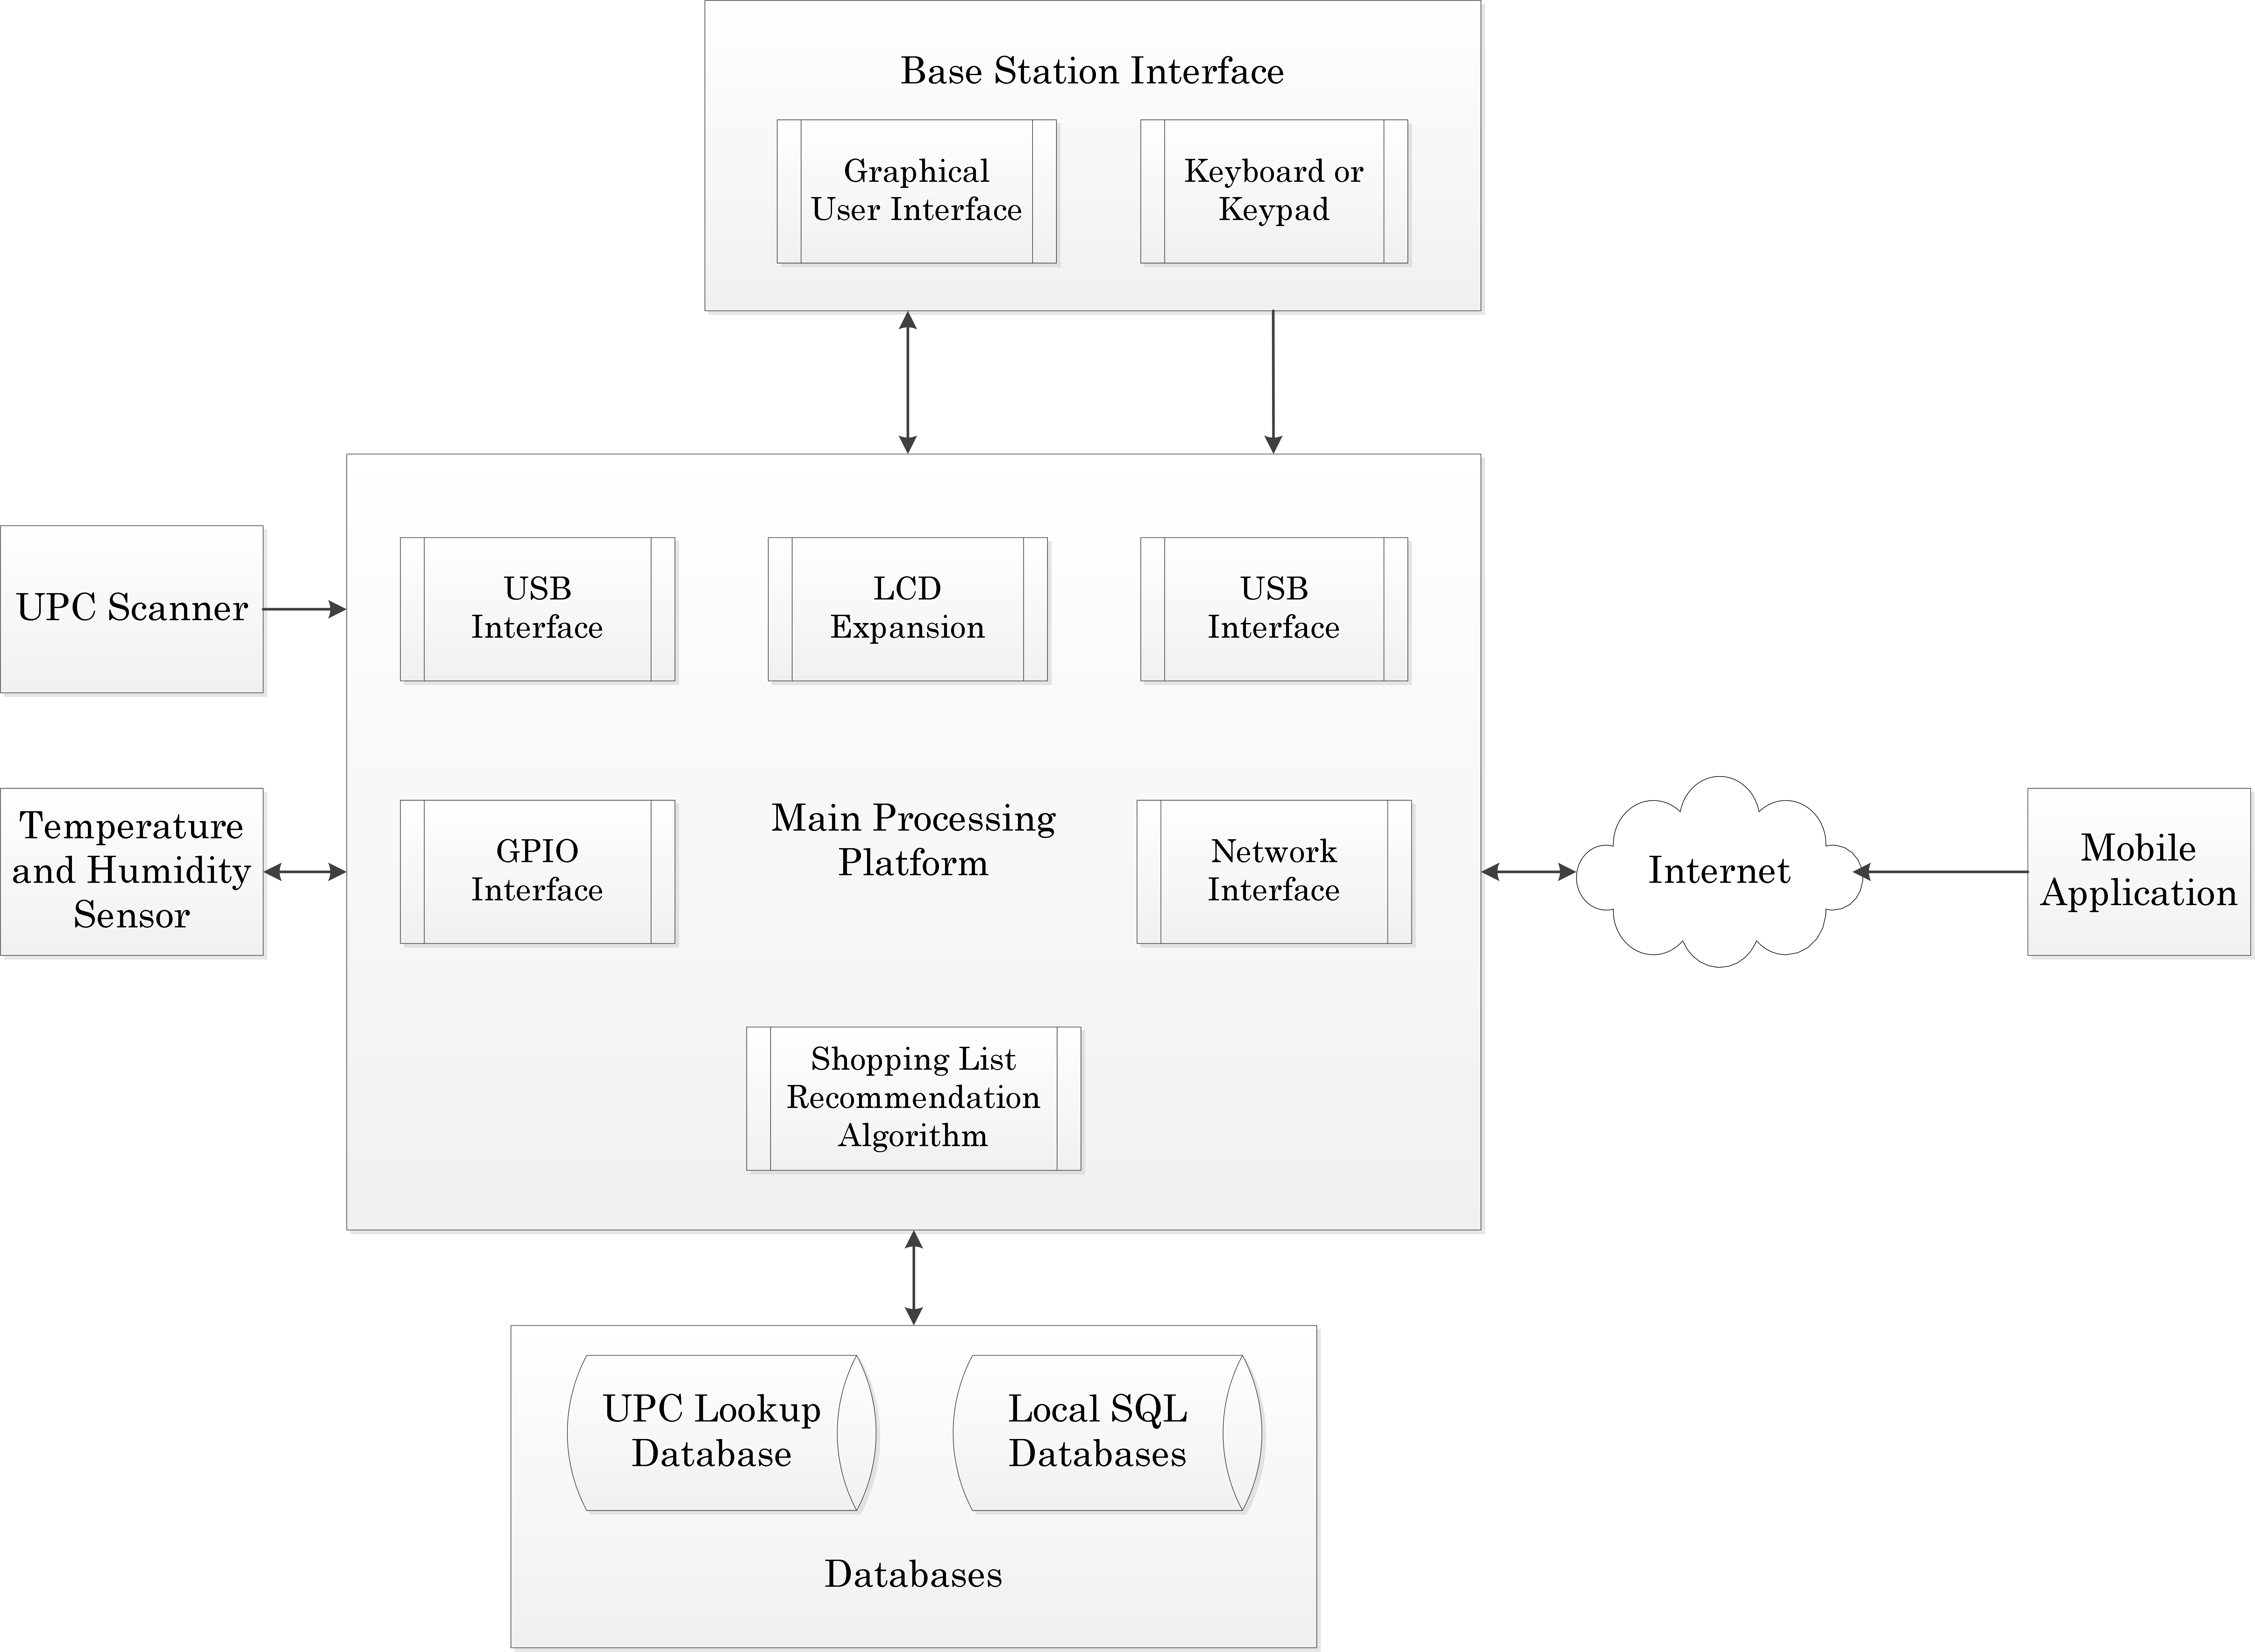
\includegraphics[scale=.3]{../Graphics/FullSystemDiagram}
\end{center}
\end{frame}

\begin{frame}{Concept Selection -- Processing Platform}
\begin{itemize}
\item Difficult to find Micro-controller with adequate peripherals / performance
\item Personal computer implementation is too general, does not fit form factor well
\item BeagleBoard offers flexibility of full Linux environment
\end{itemize}
\vspace{.5cm}
\footnotesize
\begin{tabular}{| p{.7in} | p{.7in} | p{1in} | p{0.7in} | p{.8in} | }
\cline{2-5}
\multicolumn{1}{c}{}&\multicolumn{4}{|c|}{Method} \\
\cline{2-5}
\multicolumn{1}{c|}{}&Personal \newline Computer&Tablet (Combined UI and Processing)&Micro-controller & BeagleBoard-xM\\
\hline
Processing Resources&+ + + +&+ +&+&+ + +\\
\hline
Cost &- - -& + &+ + +&+ + +\\
\hline
Size&- - -&+ +&+ + +& + + +\\
\hline
\hline
Total &2-&5+&7+& 9+\\
\hline
\end{tabular}
\end{frame}

\begin{frame}{Concept Selection -- Display}
\begin{itemize}
\item Related to choice of processing platform
\item Ideally,  ULCD7 Lite, Supported by BeagleBoard / Angstrom OS
\end{itemize}
\vspace{.5cm}
\footnotesize
\begin{tabular}{| p{1.3in} | p{.7in} | p{0.7in} | p{1.0in} | p{.8in} |}
\cline{2-4}
\multicolumn{1}{c}{}&\multicolumn{3}{|c|}{Method} \\
\cline{2-4}
\multicolumn{1}{c|}{}&LCD PC \newline Monitor&Tablet&LCD with \newline BeagleBoard-xM\\
\hline
Integration with Unit&- - -&-&+ + +\\
\hline
Ease of Use&+ + +&+ + +&+ +\\
\hline
Size of Display& + + + &+ + +&+ +\\
\hline
GUI Quality&+ + +&+ + +&+ + +\\
\hline
Size of Unit&- - -&+ + +&+ + +\\
\hline
\hline
Total&3+&12+&13+\\
\hline
\end{tabular}
\end{frame}

\begin{frame}{Concept Selection -- Expiration Date Prediction System}
\begin{itemize}
\item itemMaster UPC database provides GS1 category
\item FDA and community resources like \url{www.stilltasty.com} provide ``rule of thumb" estimates
\end{itemize}
\vspace{.5cm}
\footnotesize
\begin{tabular}{| p{.7in} | p{.7in} | p{.8in} | p{.9in} | p{.8in} |}
\cline{2-5}
\multicolumn{1}{c}{}&\multicolumn{4}{|c|}{Method} \\
\cline{2-5}
\multicolumn{1}{c|}{}&User Input \newline of expiration \newline dates& Image to Text \newline Recognition & Predictive \newline Strategy without \newline itemMaster& Predictive \newline Strategy with \newline itemMaster \\
\hline
Ease of Use&- - -&+&+ + +&+ + +\\
\hline
Feasibility&+ + +&- - -&- - -&+ + +\\
\hline
Accuracy & + + & + + &+&+\\
\hline \hline
Total &2+ &0&4+&7+\\
\hline
\end{tabular}
\end{frame}

\begin{frame}{Concept Selection -- Expiration Date Prediction System}
\begin{itemize}
\item itemMaster UPC database provides GS1 category in addition to item description
\item Number of relevant GS1 categories much small than all products, do not need to assign individual estimates of shelf life
\end{itemize}
\begin{center}
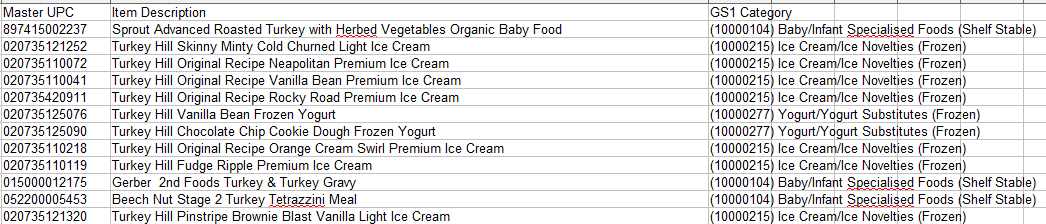
\includegraphics[scale=0.3]{../Graphics/itemMaster}
\end{center}
\end{frame}

\begin{frame}{Concept Selection -- Expiration Date Prediction System}
\begin{center}
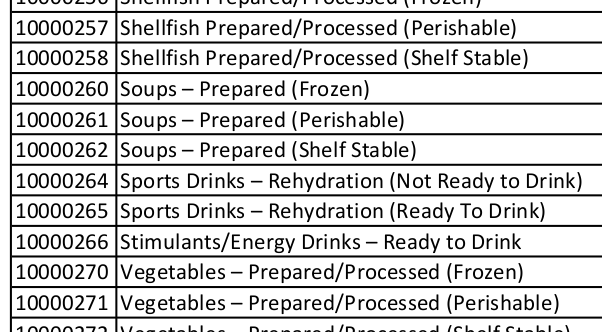
\includegraphics[scale=0.5]{../Graphics/gs1}
\end{center}
\end{frame}

\begin{frame}{Concept Selection -- Expiration Date Prediction System}
\begin{itemize}
\item There are many sources of commonly accepted shelf life estimates
\end{itemize}
\begin{center}

\includegraphics[scale=0.6]{../Graphics/stillTasty}
\newline
\vspace{1.0cm}
\newline

\includegraphics[scale=0.6]{../Graphics/fda}
\end{center}
\end{frame}

\begin{frame}{Concept Selection -- Shopping List Prediction System}
\footnotesize
\begin{tabular}{| p{1.25in} | p{.2in} | p{.8in} | p{.8in} | p{.8in} |}
\cline{3-5}
\multicolumn{2}{c}{}&\multicolumn{3}{|c|}{Method} \\
\cline{2-5}
\multicolumn{1}{c|}{}&\multicolumn{1}{|c|}{Trial}&Normal \newline Approximation&Non-Parametric \newline Distribution&Clustering to\newline produce sum of\newline Gaussians\\
\hline
\multicolumn{1}{|c|}{$\sum$ Log Probability} &1&-38.3394&-35.9682&-34.7721 \\
\cline{2-5}
\multicolumn{1}{|c|}{Observed Habits} &2&-20.5647&-17.0897&-15.6641 \\
\cline{2-5}
\multicolumn{1}{|c|}{(Goal to Maximize)} &3&-47.8101&-44.9658&-43.9845 \\
\cline{2-5}
\multicolumn{1}{|c|}{} &4&-29.1931&-19.6762&-24.4915 \\
\hline
\multicolumn{1}{|c}{Evaluation}&&- - -&-&+ + +\\
\hline
\multicolumn{1}{|c|}{$\sum$ Log Probability} &1&-36.7898&-38.4187&-50.6578\\
\cline{2-5}
\multicolumn{1}{|c|}{Habits Not} &2&-188.514&-225.002&-318.926 \\
\cline{2-5}
\multicolumn{1}{|c|}{Observed} &3&-62.2909&-63.8609&-69.9759 \\
\cline{2-5}
\multicolumn{1}{|c|}{(Goal to Minimize)} &4&-29.6667&-$\infty$&-86.0767 \\
\hline
\multicolumn{1}{|c}{Evaluation}&&- - -&+&+ +\\
\hline
\multicolumn{2}{|c|}{Ease of Computation} &+ + + &- - -&-\\
\hline \hline
\multicolumn{1}{|c}{Total}& &3- &3-&4+\\
\hline
\end{tabular}
\end{frame}

\begin{frame}{Design Overview}
\begin{itemize}
\item Project divides evenly into three task groups: the mobile application and network interface, the base station user interface and prediction system, integration of Beagleboard with peripherals and databases.
\item Base Station User Interface and Prediction System
\begin{itemize}
\item Develop GUI Application (Python 2.7 + Tkinter)
\item Expiration Data Prediction Algorithm
\item Shopping List Suggestion Algorithm
\end{itemize}
\item Mobile Application and Network Interface
\begin{itemize}
\item Develop Android Application (Java)
\item Network Interface must be robust to interrupts, and minimize data usage
\end{itemize}
\item Integration of Beagleboard with Peripherals and Databases
\begin{itemize}
\item Configure Angstrom OS Image
\item Interface with Temperature Sensor with GPIO pins (Level Shifter)
\item Scanner, keypad, display ``plug and play"
\end{itemize}
\end{itemize}
\end{frame}

\begin{frame}{Beagle Board Subsystems}
\begin{center}
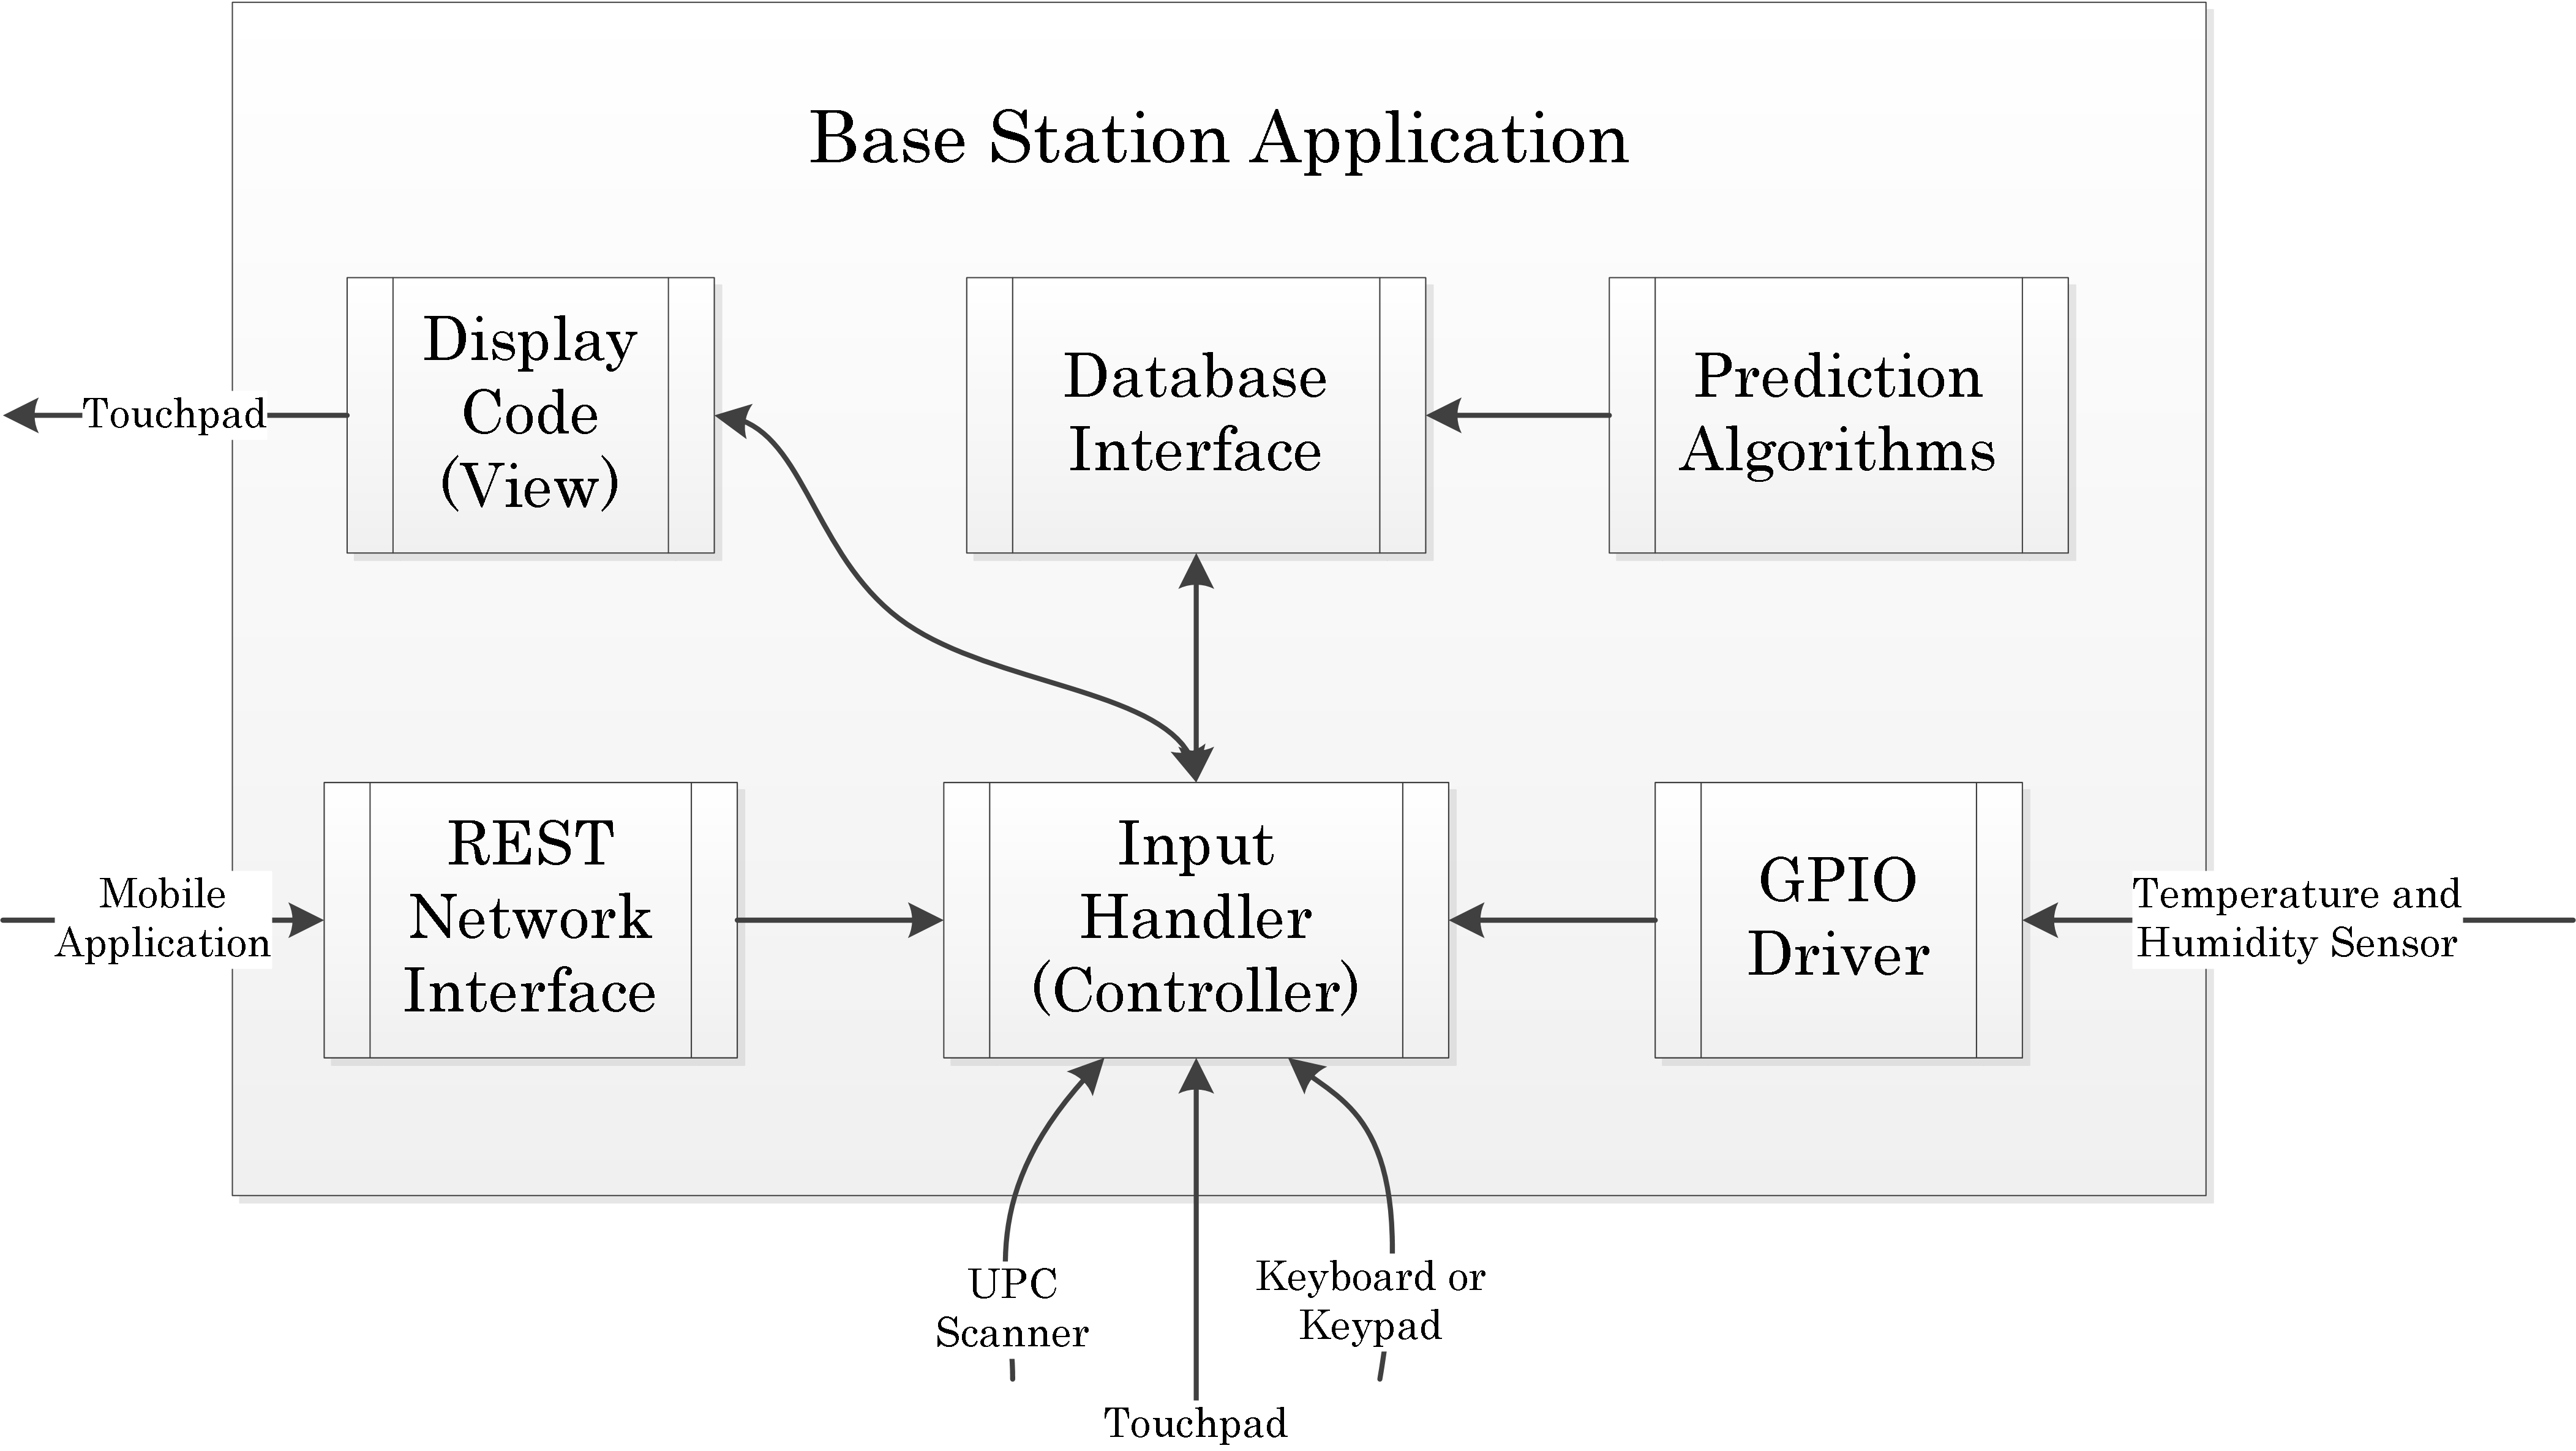
\includegraphics[scale=0.65]{../Graphics/BaseStation}
\end{center}
\end{frame}

\begin{frame}{Base Station Application}
\begin{itemize}
\item Base Station Application will be inspired by Model View Controller paradigm
\begin{itemize}
\item Input handler will be the ``Controller"
\item Combination of prediction algorithms and databases will constitute the ``Model"
\item Independent ``View", created with TkInter GUI toolkit for Python
\end{itemize}
\item Python chosen for development speed and also due to familiarity
\item SciPy scientific computing libraries will also increase speed of shopping list algorithm development
\item Will also interact with databases, some overlap of task groups will occur in this code project
\item May also handle network interface, there is an unresolved design decision between using simple custom TCP interface and using a full web-server
\end{itemize}
\end{frame}

\begin{frame}{Database Organization}
\begin{center}
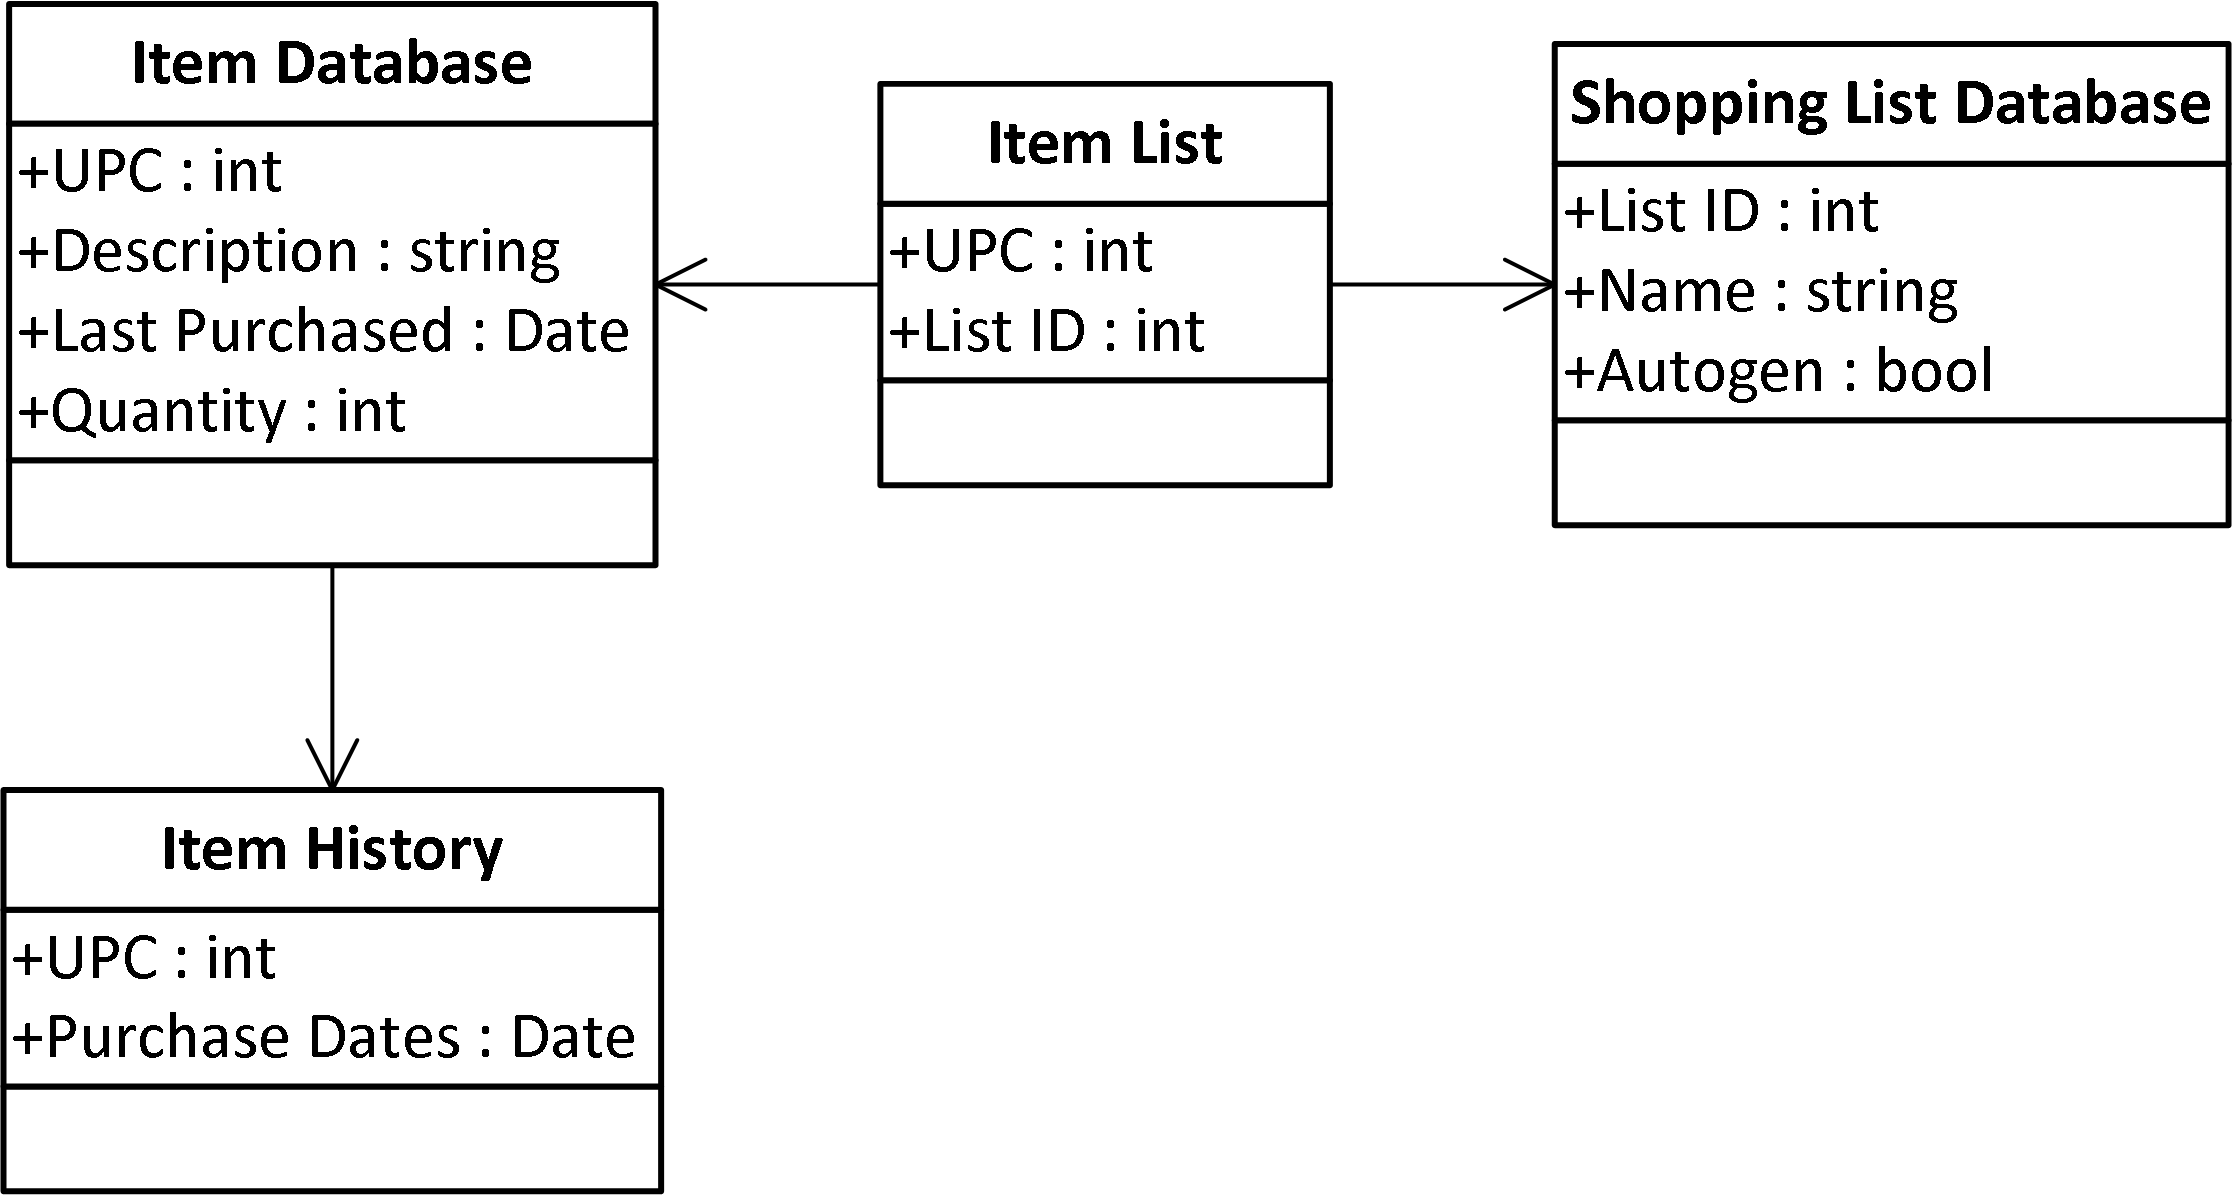
\includegraphics[scale=1.0]{../Graphics/Databases}
\end{center}
\end{frame}

\begin{frame}{User Interface Screen Captures -- Product Entry}
\begin{center}
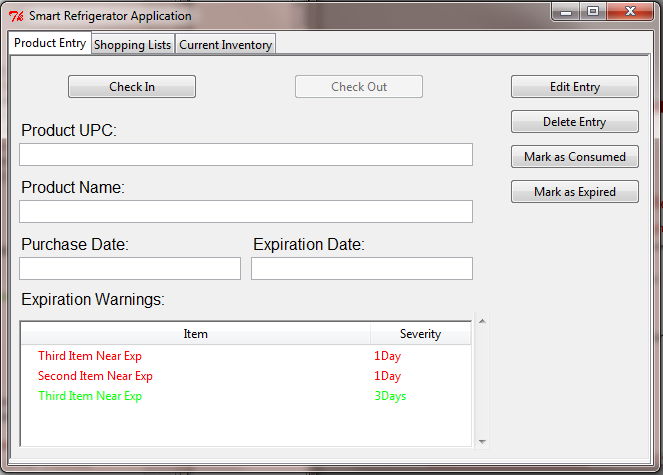
\includegraphics[scale=0.40]{../Graphics/Screenshot1}
\end{center}
\end{frame}

\begin{frame}{User Interface Screen Captures -- Shopping Lists}
\begin{center}
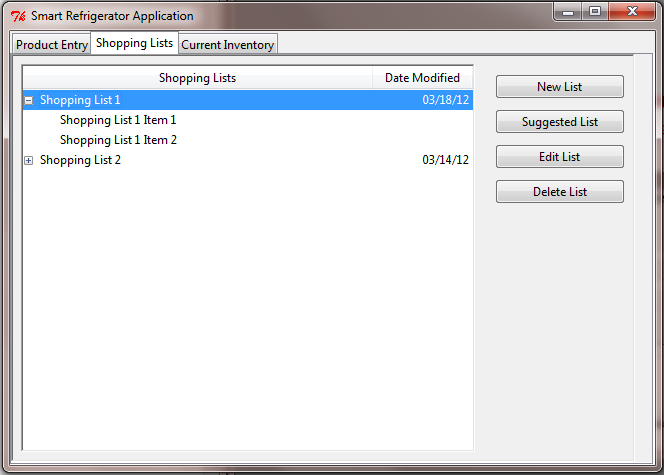
\includegraphics[scale=0.40]{../Graphics/Screenshot2}
\end{center}
\end{frame}

\begin{frame}{User Interface Screen Captures -- Shopping Lists}
\begin{center}
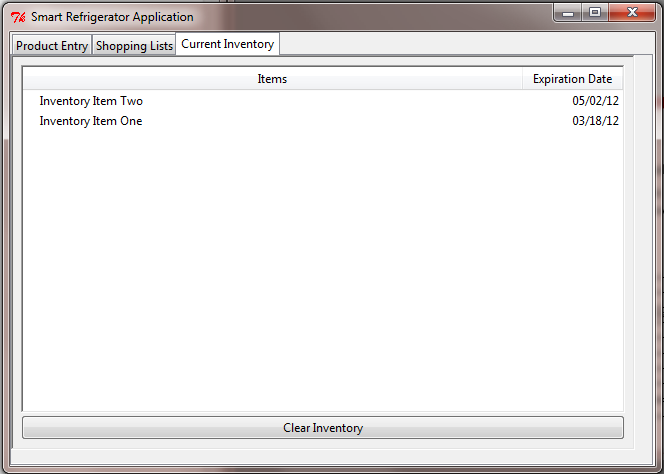
\includegraphics[scale=0.40]{../Graphics/Screenshot3}
\end{center}
\end{frame}

\begin{frame}{Mobile Interface}
\begin{itemize}
\item Mobile interface layout will be as consistent as possible with base station interface, usability benefits from consistency
\item Mobile application should limit data usage, information exchanged only on ``need to know" basis
\item Updates will not occur until specific tabs / shoppings lists selected
\item Mobile application should be tolerate of interrupted connections
\item Impact of interruptions mitigated by changing many small messages instead of monolithic ones
\end{itemize}
\end{frame}

\begin{frame}{Inventory View}
    \begin{center}
        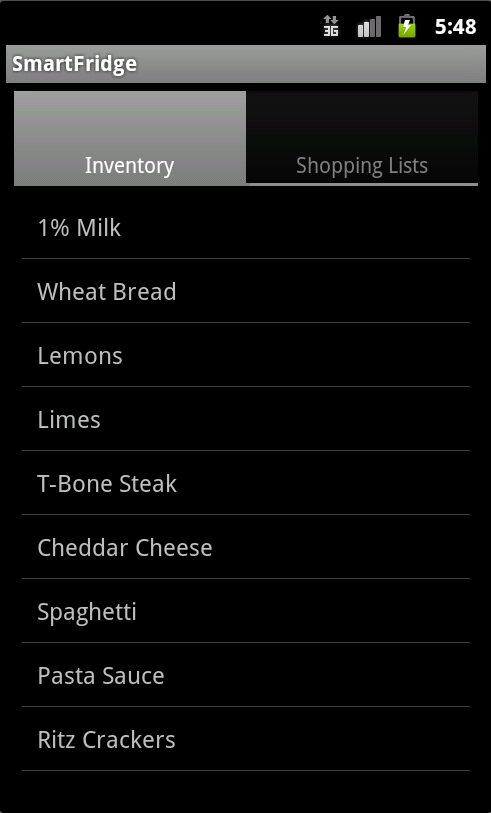
\includegraphics[scale=0.4]{../Graphics/Inventory.PNG}
    \end{center}
\end{frame}

\begin{frame}{Shopping List View}
    \begin{center}
        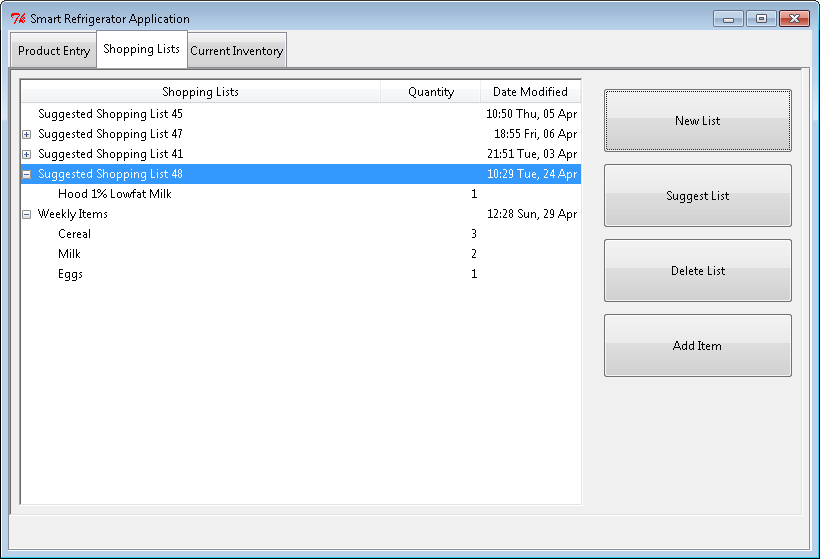
\includegraphics[scale=0.4]{../Graphics/ShoppingLists.PNG}
    \end{center}
\end{frame}

\begin{frame}{List Contents View}
    \begin{center}
        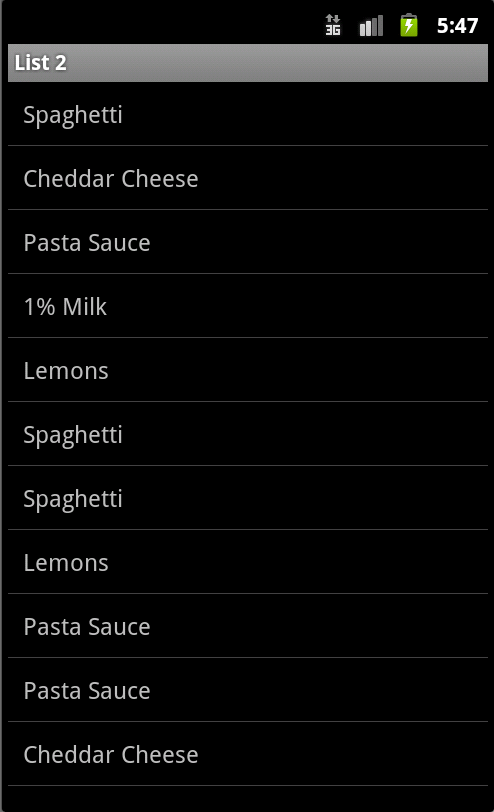
\includegraphics[scale=0.4]{../Graphics/List2_Contents.PNG}
    \end{center}
\end{frame}

\begin{frame}{Interface State Machine}
\begin{center}
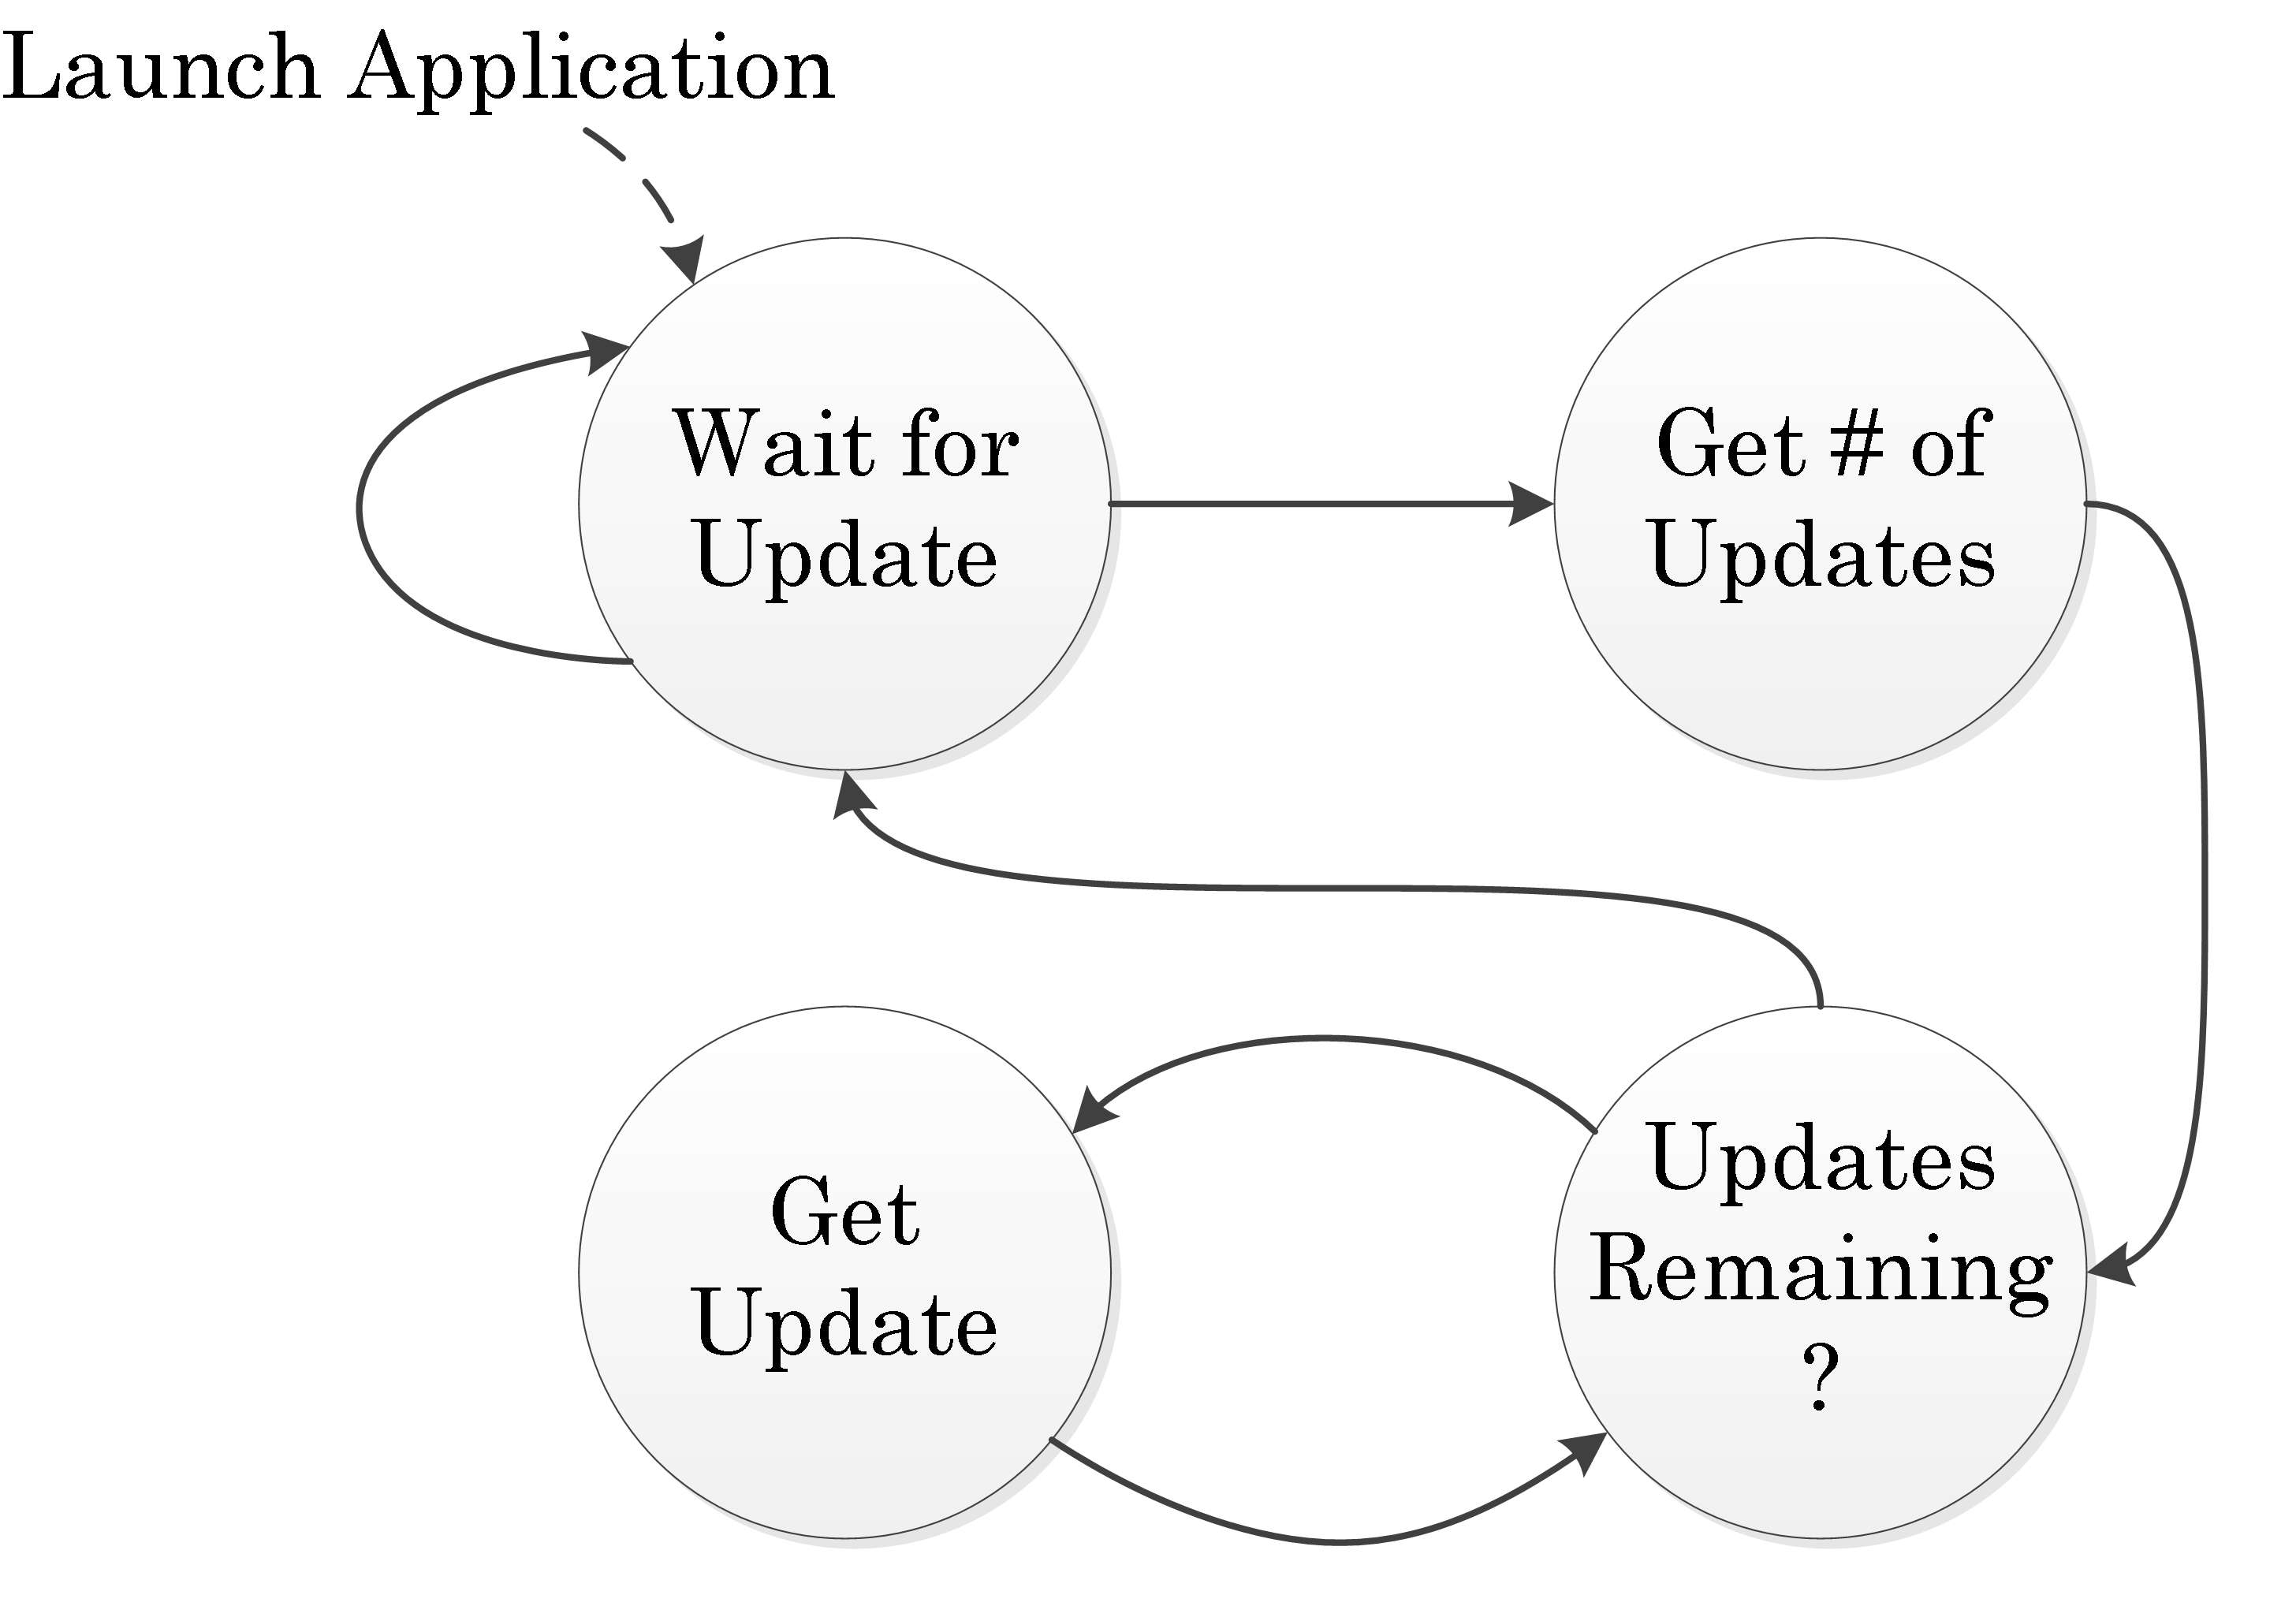
\includegraphics[scale=0.7]{../Graphics/StateMachine}
\end{center}
\end{frame}

\begin{frame}{Manufacturability, Reliability, and Background}
\begin{description}
\item[Manufacturability] - Smart Refrigerator system only a first step toward tackling food waste, could be extended to commercial systems. Prediction system could be improved by aggregating data from multiple users.
\item[Reliability] - Some components tested externally (Angstrom OS, SQL Databases). Network interface and shopping list algorithms can not be verified for all scenarios. Errors most likely in integration.
\item[Background] -
\begin{itemize}
\item Experience with Linux based operating systems critical
\item GUI development experience provided by Computer Science sequence
\item Interface to Digital Electronics useful for integrating temperature sensor
\end{itemize}
\end{description}
\end{frame}

\begin{frame}{Bill of Materials}
\begin{itemize}
\item BeagleBoard-xM provided through ARM Developer Day
\item ULCD7 Lite LCD Display hopefully will also be provided by ARM Developer Day,  though availability of this display is a significant unresolved risk
\end{itemize}
\vspace{.5cm}
\footnotesize
\begin{center}
\begin{tabular}{| p{2.0in} | p{.75in} |p{.75in} |}
\hline
Part & Retail Cost & Our Cost \\
\hline
BeagleBoard-xM & \$149 & \$0 \\
\hline
BeagleBoard-xM Power Adapter & \$14.87 & \$14.87 \\
\hline
Dorm Room Refrigerator & \$100 & \$0 \\
\hline
Android Smart Phone & \$100 & \$0  \\
\hline
LCD Display & \$80  & \$0 \\
\hline
UPC Barcode Scanner & \$35 & \$35 \\
\hline
USB Keyboard/Keypad & \$10 & \$10 \\
\hline
\hline
\textbf{Total Cost} & \$488.87 & \$59.87 \\
\hline
\end{tabular}
\end{center}
\end{frame}

\begin{frame}{Unresolved Risks -- Overview}
\begin{itemize}
\item Identified Unresolved Risks, ordered by severity:
\begin{itemize}
\item LCD Display Availability
\item Practicality of Prediction Algorithm
\item Mobile Application Data Exchange
\item Efficiency of Database Access
\end{itemize}
\end{itemize}
\end{frame}

\begin{frame}{Unresolved Risk -- LCD Display Availability}
\begin{itemize}
\item The ULCD7 Lite is the preferred choice for the display to accompany the Beagleboard. The 7-inch resistive touchscreen is designed to work with the Beagleboard and has drivers built into the Angstrom Linux distribution.
\item However, the touchscreen does not seem to be stocked by online suppliers and our request through the Arm Developer Day proposal process is still pending.
\item The BeagleBoard provides a DVI-D and S-video output, this risk could be mitigated using a traditional computer monitor if the preferred touch screen is not available.
\end{itemize}
\end{frame}

\begin{frame}{Unresolved Risk -- Practicality of Prediction Algorithm}
\begin{itemize}
\item The shopping list prediction algorithm outlined appears optimal for the test data considered. However, the analysis performed did not consider a large sample of shoppers and the conclusions drawn may not be appropriate for a larger population.
\item Also, the prediction algorithm outlined will not perform well with only a few samples; it is unclear how unacceptable this warm-up period will appear to end users.
\item The strategy presented is also quite heavy-handed and may be superfluous for this prototype system. 
\item The system will not serve as an effective shopping aid without an accurate prediction system, but a prototype may be acceptable with a much simpler system requiring significantly less effort.
\end{itemize}
\end{frame}

\begin{frame}{Unresolved Risk -- Mobile Application Data Exchange}
\begin{itemize}
\item Exchanging inventory and shopping lists data with the mobile application presents two risk areas: the amount of data plan usage required and interrupted network connections.
\item These risks are partially mitigated by the design, which exchanges data in small increments on a ``need to know" basis only, however the degree to which these risks are truly problematic is not know.
\item Interrupted connections are considered in the design, but the effectiveness of the design will be difficult to measure since it may be difficult to repeatedly interrupt the data connection.
\end{itemize}
\end{frame}

\begin{frame}{Efficiency of Database Access}
\begin{itemize}
\item Efficient practices for database access were not known or considered when partitioning information into separate tables.
\item For example, using the same database to store all possible items and the current inventory may be an inefficient choice. This strategy requires looking over all elements and extracting only those with non-zero quantities.
\item If the system was extended to large commercial applications, or if the Beagleboard was replaced with a more cost-efficient and less powerful alternative, this organization may become a significant risk.
\end{itemize}
\end{frame}

\begin{frame}{Condensed Test Plan -- Overview}
\begin{itemize}
\item Test strategy organized by subsystem:
\begin{itemize}
\item Base Station User Interface
\item Mobile User Interface and Network Interface
\item Shopping List and Expiration Prediction
\item Integration with BeagleBoard
\end{itemize}
\item Integration and System Testing
\end{itemize}
\end{frame}

\begin{frame}{Condensed Test Plan -- Base Station User Interface}
\begin{itemize}
\item The user interface is required to be easy to use and intuitive; in order to verify this someone not involved in the project should contribute to top-level testing of this sub-system.
\item Current inventory will be stored using an SQL database, test effort at this step will be verifying integration, not the storage of items.
\item The user interface must provide a notification of expiring items to the user, testing will not verify the estimate is correct, only that user interface will display notifications.
\end{itemize}
\end{frame}

\begin{frame}{Condensed Test Plan -- Mobile Application}
    \begin{itemize}
        \item Initialize a Download / Update
        \item Sever Device's network connection
        \item Reconnect Device to the network 
        \item Allow update to complete
    \end{itemize}
    Goal here is to make sure that the App will download and update inventory and grocery 
    lists through an inconsistant network connection common with mobile devices.
    \newline \quad \newline
    Other Tests:
    \begin{itemize}
        \item Usability Testing
        \item Compatibility Testing
    \end{itemize}
\end{frame}

\begin{frame}{Condensed Test Plan -- Shopping List and Expiration Prediction}
\begin{itemize}
\item Systems date must be adjustable to facilitate quick testing.
\item Enter a product code and verify that the expiration date system is initialized with recommended ``rule of thumb" value.
\item Provide feedback indicating that a product expired before estimate and validate that the estimate is decreased. Also validate the opposite case.
\item Enter a product code and advance the system time until the product is nearly expired. Verify that the prediction subsystem has indicated to controller that the product is nearing expiration.
\item Verify shoppings habits with outliers and multiple modes are modeled reasonably.
\end{itemize}
\end{frame}

\begin{frame}{Condensed Test Plan -- Integration with BeagleBoard}
\begin{itemize}
\item Verify that the BeagleBoard, with power adapter, can power all peripheral devices reliably.
\item Verify that MAC address of Ethernet interface can be statically assigned and the BeagleBoard can be pinged reliably.
\item Verify that the BeagleBoard can reliably interface with the USB scanner and USB keypad.
\item Verify that the BeagleBoard's consistently receives accurate temperature and humidity measurements from the sensor, via the general purpose input/output pins.
\item Verify that the touchscreen display accurately records users clicks and controls the pointer.
\item Verify that touchscreen accurately displays the graphical user interface without artifacts or distortion consistently, and ensure all controls on the display are accessible.
\end{itemize}
\end{frame}

\begin{frame}{Conclusion}
\LARGE
\begin{center}
Questions or Feedback?
\end{center}
\end{frame}

\begin{frame}{References}
\footnotesize
\begin{thebibliography}{9}
\bibitem{times}
Martin, Andrew. ``One Country's Table Scraps, Another Country's Meal." New York Times. N.p., 18 May 2008. Web. 26 Jan 2012. 
\url{http://www.nytimes.com/2008/05/18/weekinreview/18martin.html?pagewanted=all}.
\bibitem{lg}
Ridden, Paul. ``LG launches first Smart-Grid appliance: the Smart Fridge." gizmag. N.p., 27 Apr 2011. Web. 29 Jan 2012. \url{<http://www.gizmag.com/lg-smart-fridge/18502/>}.
\bibitem{aol}
Collins, Hugh. ``Study: US Food Waste Is a Huge Energy Drain." AolNews. N.p., 02 Oct 2010. Web. 29 Jan 2012. \url{<http://www.aolnews.com/2010/10/02/study-american-food-waste-is-a-huge-energy-drain/>}.
\bibitem{dutch}
Ramaker, Rob. ``Food waste is hard to combat." Resource. N.p., 26 Jan 2012. Web. 29 Jan 2012. \url{<http://resource.wur.nl/en/wetenschap/detail/food_waste_is_hard_to_combat/>}.
 \end{thebibliography}
\end{frame}

\end{document}


